% OmniLaTeX — Overleaf Template
% Compile with: LuaLaTeX (Menu → Compiler → LuaLaTeX)
%
% ─────────────────────────────────────────────────────────
% OmniLaTeX is a modular document class that adapts to any
% document type. Change one option to switch profiles.
% ─────────────────────────────────────────────────────────
%
% Full documentation: https://github.com/WyattAu/OmniLaTeX-template

%!TEX TS-program = lualatex

% ── Document Class ──────────────────────────────────────
% Change `doctype` to switch document profiles:
%
%   doctype=thesis            Academic thesis (scrbook)
%   doctype=dissertation      Doctoral dissertation (scrbook)
%   doctype=book              Book or monograph (scrbook)
%   doctype=dictionary        Dictionary or lexicon (scrbook)
%   doctype=technicalreport   Technical report (scrreprt)
%   doctype=report            General report (scrreprt)
%   doctype=standard          Standards document (scrreprt)
%   doctype=patent            Patent application (scrreprt)
%   doctype=manual            Manual or handbook (scrreprt)
%   doctype=article           Article or paper (scrartcl)
%   doctype=journal           Journal article (scrartcl)
%   doctype=inlinepaper       Inline research paper (scrartcl)
%   doctype=cv                Curriculum vitae (scrartcl)
%   doctype=cover-letter      Cover letter (scrartcl)
%   doctype=letter            Formal letter (scrartcl)
%   doctype=poster            Conference poster (scrartcl)
%   doctype=presentation      Presentation slides (scrartcl)
%
% Change `language` to set the document language:
%   english, german, french, spanish, portuguese, italian,
%   dutch, russian, chinese, japanese, korean, arabic
%
% Add `institution=NAME` for institutional branding:
%   tuhh, tum, eth, mit, stanford, cambridge, tudelft, generic

\documentclass[
  doctype=thesis,
  language=english,
  institution=none,
]{omnilatex}

% ── Bibliography ────────────────────────────────────────
% Add your .bib file(s) here:
% \addbibresource{bib/bibliography.bib}

% ── Metadata ────────────────────────────────────────────
\title{My Thesis Title}
\subtitle{An Optional Subtitle}
\author{Author Name}
\date{\today}

% ── Custom Commands (optional) ──────────────────────────
% \newcommand{\keyword}[1]{\textbf{\textcolor{blue}{#1}}}

\begin{document}

\maketitle
\tableofcontents

% ═══════════════════════════════════════════════════════
%  Chapter 1: Introduction
% ═══════════════════════════════════════════════════════

\chapter{Introduction}

This is the OmniLaTeX template for Overleaf. It demonstrates the
most common features you'll use when writing academic documents.

OmniLaTeX is built on LuaLaTeX and KOMA-Script. It provides a single
document class that adapts to 16 document profiles via 55 aliases.

\section{Why OmniLaTeX}

Instead of maintaining separate templates for each document type,
OmniLaTeX lets you switch by changing one option:

\begin{verbatim}
\documentclass[doctype=article]{omnilatex}
\end{verbatim}

% ═══════════════════════════════════════════════════════
%  Chapter 2: Features
% ═══════════════════════════════════════════════════════

\chapter{Features}

\section{Mathematics}

Inline math: $E = mc^2$. Display math:

\begin{equation}
  \int_{-\infty}^{\infty} e^{-x^2} \, dx = \sqrt{\pi}
  \label{eq:gaussian}
\end{equation}

Refer to equations with \verb|\eqref{}|: Equation~\eqref{eq:gaussian}.

\section{Tables}

\begin{table}[htbp]
  \centering
  \caption{Sample comparison of document profiles}
  \label{tab:profiles}
  \begin{tabular}{lcc}
    \toprule
    \textbf{Profile} & \textbf{Base Class} & \textbf{Sides} \\
    \midrule
    Thesis            & scrbook  & Two-sided \\
    Technical Report  & scrreprt & Two-sided \\
    Article           & scrartcl & One-sided  \\
    CV                & scrartcl & One-sided  \\
    \bottomrule
  \end{tabular}
\end{table}

\section{Figures}

\begin{figure}[htbp]
  \centering
  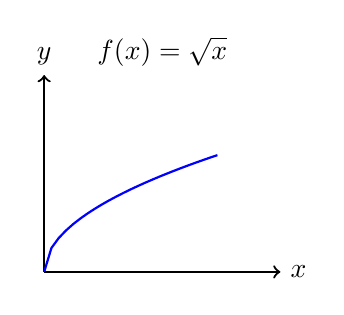
\begin{tikzpicture}
    \draw[thick, ->] (0,0) -- (3,0) node[right] {$x$};
    \draw[thick, ->] (0,0) -- (0,2.5) node[above] {$y$};
    \draw[blue, thick, domain=0:2.2] plot (\x, {sqrt(\x)});
    \node at (1.5,2.8) {$f(x) = \sqrt{x}$};
  \end{tikzpicture}
  \caption{Example TikZ figure}
  \label{fig:example}
\end{figure}

% For external images:
% \begin{figure}[htbp]
%     \centering
%     \includegraphics[width=0.8\textwidth]{assets/images/photo.jpg}
%     \caption{Your image caption}
%     \label{fig:photo}
% \end{figure}

\section{Code Listings}

\begin{listing}[htbp]
  \begin{minted}{python}
def fibonacci(n: int) -> list[int]:
    """Compute the first n Fibonacci numbers."""
    a, b = 0, 1
    result = []
    for _ in range(n):
        result.append(a)
        a, b = b, a + b
    return result

print(fibonacci(10))
  \end{minted}
  \caption{Fibonacci sequence in Python}
  \label{lst:fibonacci}
\end{listing}

% ═══════════════════════════════════════════════════════
%  Chapter 3: Methodology
% ═══════════════════════════════════════════════════════

\chapter{Methodology}

Write your methodology here. Use sections and subsections to organize:

\section{Experimental Setup}

\begin{enumerate}
  \item First step
  \item Second step
  \item Third step
\end{enumerate}

\section{Results}

\begin{itemize}
  \item Key finding A
  \item Key finding B
  \item Key finding C
\end{itemize}

% ═══════════════════════════════════════════════════════
%  Chapter 4: Conclusion
% ═══════════════════════════════════════════════════════

\chapter{Conclusion}

Summarize your findings and contributions here.

% ── Bibliography ────────────────────────────────────────
% Uncomment when you have citations:
% \printbibliography[heading=bibintoc]

\end{document}
